\section{Fortran程序结构}
\subsection{Fortran程序构成和子程序}

\subsubsection{Fortran程序基本构成}
Fortran程序一般由以下几个部分构成：
\begin{itemize}
      \item 程序头：包括程序名、变量声明等。
      \item 主程序：包含程序的主要逻辑和计算部分。
      \item 子程序：可选部分，用于实现特定功能的代码块。
      \item 结束语句：标志程序的结束。
\end{itemize}
例如：
\begin{envcode}{fortran}{Fortran}
      PROGRAM HelloWorld
      INTEGER :: I
      REAL :: X, Y
      
      WRITE(6, '(A)') 'Hello, World!'
      
      I = 5
      X = 3.14
      Y = 2.718281828459045
      
      WRITE(6, '(I5, F10.2, E10.3)') I, X, Y
      
      END PROGRAM HelloWorld
\end{envcode}

其中第一行\code{PROGRAM HelloWorld}表示程序名为\code{HelloWorld}，非必需，可以不写。

接下来是变量声明部分，使用\code{INTEGER}和\code{REAL}声明了整数和实数类型的变量，这里的内容实际上包含在隐式声明内了，可以不再显式声明。

\code{END}语句标志程序的结束，后面的\code{PROGRAM HelloWorld}表示程序名的结束，也可以直接写\code{END}。

\subsubsection{函数子程序（FUNCTION）}

用于计算并返回单个主值，可通过形参额外传递多个值；
\textbf{函数名必须赋值}，调用方式与库函数一致（直接写在算术表达式中）。

例如，计算二项式系数$C(n,i) = \frac{n!}{i!(n-i)!}$，发现其中有大量阶乘的计算，
则可编写一个阶乘的函数子程序文件\code{ifact.f}：
\begin{envcode}{fortran}{Fortran}
C FUNCTION SUBPROGRAM: COMPUTE K FACTORIAL
      FUNCTION IFACT(K)
      INTEGER IFACT, K, J
      IFACT = 1
      IF(K.EQ.0) RETURN
      DO 10 J = 1, K
          IFACT = IFACT * J
10    CONTINUE
      RETURN
      END
\end{envcode}
其中\code{RETURN}语句用于返回函数值，函数名\code{IFACT}即为返回值变量。

主程序文件\code{binom.f}即可调用该函数：
\begin{envcode}{fortran}{Fortran}
C MAIN PROGRAM: CALCULATE BINOMIAL COEFFICIENT
      INTEGER UP, DOWN, IBINQ, N, I
      READ(5, *) N, I
      UP = IFACT(N)
      DOWN = IFACT(N-I) * IFACT(I)
      IBINQ = UP / DOWN
      WRITE(6, 20) N, I, IBINQ
20    FORMAT(6X, 'N=', I5, 5X, 'I=', I5, 5X, 'BINOMIAL COEFF=', I8)
      STOP
      END
\end{envcode}

编译并运行测试：
\begin{envcode}{console}{Bash}
user1@host:~/learn$ gfortran -c binom.f ifact.f
user1@host:~/learn$ gfortran -o binom binom.o ifact.o
user1@host:~/learn$ ./binom
8,3
      N=    8     I=    3     BINOMIAL COEFF=      56
\end{envcode}

\subsubsection{过程子程序（SUBROUTINE）}
用于计算多个值或执行特定任务（如交换变量、数组排序）；
\textbf{子程序名无需赋值}，必须通过\code{CALL}语句调用。

例如，编写一个交换两个数的子程序文件\code{swap.f}：
\begin{envcode}{fortran}{Fortran}
C SUBROUTINE TO SWAP TWO NUMBERS
      SUBROUTINE SWAP(A, B)
      REAL :: A, B, TEMP
      TEMP = A
      A = B
      B = TEMP
      RETURN
      END
\end{envcode}
主程序文件\code{testswap.f}即可调用该子程序：
\begin{envcode}{fortran}{Fortran}
C MAIN PROGRAM: CALL INTCHG TO SWAP TWO NUMBERS
      REAL A, B
      A = 5.5
      B = 10.2
      WRITE(6, 10) A, B
10    FORMAT(1X, 'BEFORE SWAP: A=', F5.1, 2X, 'B=', F5.1)
      CALL INTCHG(A, B)
      WRITE(6, 20) A, B
20    FORMAT(1X, 'AFTER SWAP: A=', F5.1, 2X, 'B=', F5.1)
      STOP
      END
\end{envcode}

编译并运行测试：
\begin{envcode}{console}{Bash}
user1@host:~/learn$ gfortran -c testswap.f swap.f
user1@host:~/learn$ gfortran -o testswap testswap.o swap.o
user1@host:~/learn$ ./testswap
BEFORE SWAP: A= 5.5  B=10.2
AFTER SWAP: A=10.2  B= 5.5
\end{envcode}

\subsubsection{算术语句函数}

如可在主程序内直接定义函数$G(x)=x^2-5x+2$，并计算$x=1\sim{}20$：
\begin{envcode}{fortran}{Fortran}
C MAIN PROGRAM WITH ARITHMETIC STATEMENT FUNCTION
      REAL G, X, VALUE
      INTEGER J
C DEFINE STATEMENT FUNCTION
      G(X) = X*X - 5.0*X + 2.0
C CALCULATE AND PRINT VALUES
      DO 100 J = 1, 20
          X = FLOAT(J)
          VALUE = G(X)
          WRITE(6, 10) J, VALUE
10        FORMAT(1X, 'X=', I3, 2X, 'G(X)=', F8.2)
100   CONTINUE
      STOP
      END
\end{envcode}

编译后运行测试：
\begin{envcode}{console}{Bash}
user1@host:~/learn$ ./statfunc
X=  1  G(X)=  -2.00
X=  2  G(X)=  -4.00
X=  3  G(X)=  -4.00
X=  4  G(X)=  -2.00
· · ·
\end{envcode}

\begin{zj}
FUNCTION和SUBROUTINE子程序

如上所示，Fortran程序的构成和子程序的使用非常灵活，可以根据需要编写不同的子程序来实现特定的功能。

其中函数子程序与函数使用方法相同，用于计算并返回单个主值。

过程子程序相当于“插入”一段关于过程，用于执行特定任务或计算多个值。

无论是函数子程序还是过程子程序，都可以通过形参传递多个值，实现更复杂的计算和功能。
形参就是在子程序定义时使用的变量名，用于接收调用时传递的实际参数值。

二者在定义时，都需要声明变量或数组的类型和维数，以确保正确处理传递的数据。
\end{zj}

\subsection{程序框图}
程序框图是一种用于表示程序逻辑结构的图形工具，通过不同的符号和连接线来表示程序的各个部分及其关系。常用的程序框图符号包括：
\begin{itemize}
      \item 起始/结束符号：表示程序的开始和结束，通常用椭圆形表示。
      \item 处理符号：表示程序中的处理步骤，如计算、赋值等，通常用矩形表示。
      \item 输入/输出符号：表示程序中的输入和输出操作，通常用平行四边形表示。
      \item 决策符号：表示程序中的条件判断，通常用菱形表示。
      \item 连接线：表示程序流程的方向，连接各个符号。
\end{itemize}
通过程序框图，可以清晰地展示程序的逻辑结构和流程。例如，下面是一个简单的程序框图（图\ref{fig:program_flowchart}），表示一个循环结构的程序。
\begin{figure}[ht]
      \centering
      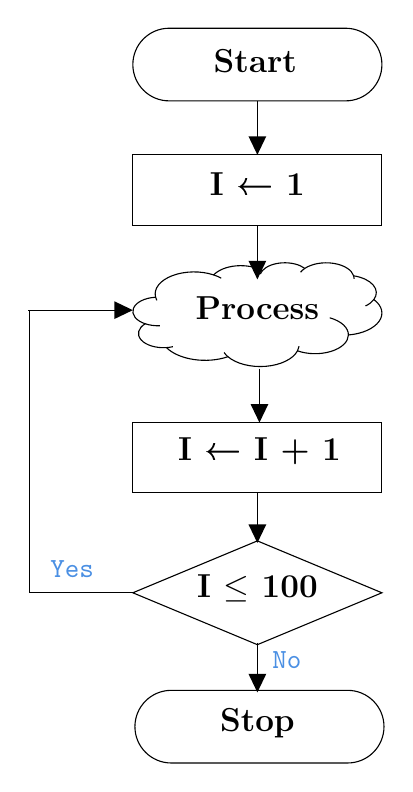
\begin{tikzpicture}[x=0.75pt,y=0.75pt,yscale=-1,xscale=1]
      %uncomment if require: \path (0,385); %set diagram left start at 0, and has height of 385

      %Rounded Rect [id:dp8328588102090151] 
      \draw   (290,34.5) .. controls (290,24.84) and (297.84,17) .. (307.5,17) -- (392.5,17) .. controls (402.16,17) and (410,24.84) .. (410,34.5) -- (410,34.5) .. controls (410,44.16) and (402.16,52) .. (392.5,52) -- (307.5,52) .. controls (297.84,52) and (290,44.16) .. (290,34.5) -- cycle ;
      %Shape: Rectangle [id:dp17985251419884474] 
      \draw   (290,78) -- (410,78) -- (410,111.83) -- (290,111.83) -- cycle ;
      %Straight Lines [id:da13836301690190234] 
      \draw    (350,52) -- (350,75) ;
      \draw [shift={(350,78)}, rotate = 270] [fill={rgb, 255:red, 0; green, 0; blue, 0 }  ][line width=0.08]  [draw opacity=0] (8.93,-4.29) -- (0,0) -- (8.93,4.29) -- cycle    ;
      %Shape: Cloud [id:dp22782610661330427] 
      \draw   (300.92,146.46) .. controls (299.95,142.43) and (303.13,138.44) .. (309.09,136.18) .. controls (315.06,133.93) and (322.77,133.8) .. (328.95,135.86) .. controls (331.14,133.51) and (335.15,131.89) .. (339.77,131.49) .. controls (344.39,131.09) and (349.07,131.95) .. (352.4,133.81) .. controls (354.26,131.68) and (357.93,130.25) .. (362.09,130.03) .. controls (366.25,129.81) and (370.33,130.82) .. (372.86,132.71) .. controls (376.23,130.46) and (381.6,129.51) .. (386.64,130.27) .. controls (391.67,131.04) and (395.47,133.38) .. (396.4,136.29) .. controls (400.53,136.93) and (403.97,138.56) .. (405.83,140.75) .. controls (407.7,142.94) and (407.8,145.49) .. (406.11,147.72) .. controls (410.18,150.73) and (411.13,154.74) .. (408.61,158.25) .. controls (406.09,161.76) and (400.48,164.24) .. (393.87,164.78) .. controls (393.82,168.07) and (390.64,171.1) .. (385.54,172.68) .. controls (380.45,174.27) and (374.25,174.17) .. (369.32,172.43) .. controls (367.22,176.37) and (361.31,179.28) .. (354.15,179.88) .. controls (346.98,180.49) and (339.85,178.69) .. (335.82,175.26) .. controls (330.89,176.95) and (324.96,177.44) .. (319.39,176.61) .. controls (313.82,175.79) and (309.07,173.72) .. (306.2,170.87) .. controls (301.16,171.21) and (296.29,169.73) .. (294,167.16) .. controls (291.71,164.59) and (292.49,161.49) .. (295.96,159.4) .. controls (291.47,157.89) and (289.17,154.91) .. (290.27,152) .. controls (291.38,149.1) and (295.63,146.92) .. (300.82,146.62) ; \draw   (295.97,159.39) .. controls (298.09,160.1) and (300.54,160.43) .. (302.99,160.32)(306.21,170.87) .. controls (307.26,170.8) and (308.29,170.66) .. (309.28,170.43)(335.82,175.26) .. controls (335.08,174.63) and (334.45,173.96) .. (333.97,173.25)(369.32,172.43) .. controls (369.7,171.71) and (369.95,170.97) .. (370.06,170.22)(393.86,164.78) .. controls (393.91,161.27) and (390.41,158.06) .. (384.84,156.52)(406.11,147.72) .. controls (405.21,148.92) and (403.83,149.98) .. (402.09,150.82)(396.4,136.29) .. controls (396.55,136.77) and (396.62,137.26) .. (396.61,137.75)(372.86,132.71) .. controls (372.02,133.27) and (371.33,133.9) .. (370.8,134.57)(352.4,133.81) .. controls (351.95,134.32) and (351.61,134.86) .. (351.4,135.42)(328.95,135.86) .. controls (330.26,136.29) and (331.47,136.81) .. (332.56,137.42)(300.92,146.46) .. controls (301.05,147.02) and (301.26,147.57) .. (301.55,148.1) ;
      %Straight Lines [id:da7840256672973447] 
      \draw    (350,112) -- (350,135) ;
      \draw [shift={(350,138)}, rotate = 270] [fill={rgb, 255:red, 0; green, 0; blue, 0 }  ][line width=0.08]  [draw opacity=0] (8.93,-4.29) -- (0,0) -- (8.93,4.29) -- cycle    ;
      %Shape: Rectangle [id:dp20472903555734168] 
      \draw   (290,207) -- (410,207) -- (410,240.83) -- (290,240.83) -- cycle ;
      %Straight Lines [id:da2618437898650212] 
      \draw    (351,181) -- (351,204) ;
      \draw [shift={(351,207)}, rotate = 270] [fill={rgb, 255:red, 0; green, 0; blue, 0 }  ][line width=0.08]  [draw opacity=0] (8.93,-4.29) -- (0,0) -- (8.93,4.29) -- cycle    ;
      %Shape: Diamond [id:dp6500945499785862] 
      \draw   (350,264) -- (410,289) -- (350,314) -- (290,289) -- cycle ;
      %Straight Lines [id:da316528847526659] 
      \draw    (350,241) -- (350,262) ;
      \draw [shift={(350,265)}, rotate = 270] [fill={rgb, 255:red, 0; green, 0; blue, 0 }  ][line width=0.08]  [draw opacity=0] (8.93,-4.29) -- (0,0) -- (8.93,4.29) -- cycle    ;
      %Shape: Right Angle [id:dp35661600831744167] 
      \draw   (290,288.83) -- (240,288.83) -- (240,152.83) ;
      %Rounded Rect [id:dp12383134692351772] 
      \draw   (291,353.5) .. controls (291,343.84) and (298.84,336) .. (308.5,336) -- (393.5,336) .. controls (403.16,336) and (411,343.84) .. (411,353.5) -- (411,353.5) .. controls (411,363.16) and (403.16,371) .. (393.5,371) -- (308.5,371) .. controls (298.84,371) and (291,363.16) .. (291,353.5) -- cycle ;
      %Straight Lines [id:da1422568232591901] 
      \draw    (350,313) -- (350,334) ;
      \draw [shift={(350,337)}, rotate = 270] [fill={rgb, 255:red, 0; green, 0; blue, 0 }  ][line width=0.08]  [draw opacity=0] (8.93,-4.29) -- (0,0) -- (8.93,4.29) -- cycle    ;
      %Straight Lines [id:da26294265696172126] 
      \draw    (239.6,152.83) -- (287,152.83) ;
      \draw [shift={(290,152.83)}, rotate = 180] [fill={rgb, 255:red, 0; green, 0; blue, 0 }  ][line width=0.08]  [draw opacity=0] (8.93,-4.29) -- (0,0) -- (8.93,4.29) -- cycle    ;

      % Text Node
      \draw (349,32.92) node   [align=left] {\begin{minipage}[lt]{81.6pt}\setlength\topsep{0pt}
      \begin{center}
      \textbf{{\large {Start}}}
      \end{center}

      \end{minipage}};
      % Text Node
      \draw (350,91.92) node   [align=left] {\begin{minipage}[lt]{81.6pt}\setlength\topsep{0pt}
      \begin{center}
      {\large \textbf{I ← 1}}
      \end{center}

      \end{minipage}};
      % Text Node
      \draw (350,151.92) node   [align=left] {\begin{minipage}[lt]{81.6pt}\setlength\topsep{0pt}
      \begin{center}
      {\large \textbf{Process}}
      \end{center}

      \end{minipage}};
      % Text Node
      \draw (351,220.92) node   [align=left] {\begin{minipage}[lt]{81.6pt}\setlength\topsep{0pt}
      \begin{center}
      {\textbf{{\large I ← I + 1}}}
      \end{center}

      \end{minipage}};
      % Text Node
      \draw (350,287) node   [align=left] {\begin{minipage}[lt]{81.6pt}\setlength\topsep{0pt}
      \begin{center}
      {\textbf{{\large I $\leq$ 100}}}
      \end{center}

      \end{minipage}};
      % Text Node
      \draw (249,272) node [anchor=north west][inner sep=0.75pt]   [align=left] {{\texttt{\textcolor[rgb]{0.29,0.56,0.89}{Yes}}}};
      % Text Node
      \draw (350,351.92) node   [align=left] {\begin{minipage}[lt]{81.6pt}\setlength\topsep{0pt}
      \begin{center}
      \textbf{{\large Stop}}
      \end{center}

      \end{minipage}};
      % Text Node
      \draw (356,316) node [anchor=north west][inner sep=0.75pt]   [align=left] {{\texttt{\textcolor[rgb]{0.29,0.56,0.89}{No}}}};


      \end{tikzpicture}

      \caption{循环结构的程序框图}
      \label{fig:program_flowchart}
\end{figure}

程序框图能够帮助程序员更好地理解和设计程序逻辑，提高程序的可读性和维护性。在编写复杂程序时，建议先绘制程序框图，以便理清思路，确保程序逻辑的正确性。
笔记中绘制程序框图比较麻烦，固本笔记之后不再展示程序框图。

\subsection{IF语句}

\subsubsection{条件表达式}
条件表达式用于判断某个条件是否成立。在Fortran中，条件表达式通常由关系运算符和逻辑运算符组成。常见的关系运算符包括：
\begin{itemize}
    \item \code{.GT.}：大于
    \item \code{.LT.}：小于
    \item \code{.EQ.}：等于
    \item \code{.NE.}：不等于
    \item \code{.GE.}：大于等于
    \item \code{.LE.}：小于等于
\end{itemize}

除此之外，条件表达还能利用逻辑运算符进行组合，常见的逻辑运算符包括：
\begin{itemize}
    \item \code{.AND.}：逻辑与（二者均为真）
    \item \code{.OR.}：逻辑或（至少一个为真）
\end{itemize}

\subsubsection{IF语句结构}
\code{IF}语句用于实现条件判断和分支执行。Fortran中有多种形式的\code{IF}语句，常见的包括单行IF语句、块IF语句、多层级IF语句、算数\code{IF}语句等。
单行IF语句用于在条件满足时执行一条语句，例如：
\begin{envcode}{fortran}{Fortran}
      IF(X.GT.0) WRITE(6,*)X,Y
\end{envcode}

块IF语句用于在条件满足时执行多条语句，例如：
\begin{envcode}{fortran}{Fortran}
      IF(X.GT.0) THEN
          Y = X**2
          WRITE(6,*)Y
      ENDIF
\end{envcode}

多层级\code{IF}语句用于在一个\code{IF}语句内部包含多个分支，例如：
\begin{envcode}{fortran}{Fortran}
      IF(X.GT.0) THEN
          IF(Y.LT.0) THEN
              Z = X + Y
          ELSE
              Z = X - Y
          ENDIF
      ENDIF
\end{envcode}

算数\code{IF}语句用于根据表达式的值选择执行的分支，表达式的值小于、等于、大于零，分别执行其后指定的三个语句，例如：
\begin{envcode}{fortran}{Fortran}
      IF(X) 10, 20, 30
10    WRITE(6,*) 'X < 0'
20    WRITE(6,*) 'X = 0'
30    WRITE(6,*) 'X > 0'
\end{envcode}

除此之外，\code{IF}语句还能嵌套使用，实现更复杂的条件判断和分支执行。

\begin{zy}
IF语句中的条件表达式注意事项

若变量为浮点数时，尽量不要使用\code{.EQ.}和\code{.NE.}进行比较，因为浮点数的精度问题可能导致判断不准确。建议使用范围判断或其他方法进行比较。
如要判断浮点数是否接近某个值，可以使用绝对误差的方式，例如：
\begin{envcode}{fortran}{Fortran}
      IF(ABS(X - TARGET).LT..00001) THEN
          ...
      ENDIF
\end{envcode}

注意，“\code{.LT..00001}”中，前两个点是运算符的一部分，后一个点是小数点，是\code{0.00001}的省略表示方法。
\end{zy}

\subsection{GOTO语句}
\code{GOTO}语句用于无条件地跳转到程序中的指定标签位置。标签是一个整数，通常位于程序行的开头，用于标识程序中的某个位置。使用\code{GOTO}语句可以实现程序流程的跳转，但过度使用可能导致程序结构混乱，降低可读性。
例如，可以利用\code{GOTO}语句和\code{IF}语句实现一个简单的循环：
\begin{envcode}{fortran}{Fortran}
      INTEGER I
      I = 1
10    CONTINUE
      IF(I.GT.100) GOTO 20
      I = I + 1
      GOTO 10
20    CONTINUE
      END
\end{envcode}

也可以不用\code{CONTINUE}语句，直接使用标签：
\begin{envcode}{fortran}{Fortran}
      INTEGER I
      I = 1
10    IF(I.GT.100) GOTO 20
      I = I + 1
      GOTO 10
20    END
\end{envcode}

由此可见，可以利用\code{GOTO}造成循环，再结合\code{IF}语句实现条件跳转，从而控制跳出循环。

还有一种选择结构的实现方式，即利用\code{GOTO}语句实现多分支选择：
\begin{envcode}{fortran}{Fortran}
      GOTO (10, 20, 30) N
10    WRITE(6,*) 'N = 1'
20    WRITE(6,*) 'N = 2'
30    WRITE(6,*) 'N = 3'
      END
\end{envcode}

\begin{zy}
GOTO语句的使用

虽然\code{GOTO}语句可以实现程序流程的跳转，但过度使用可能导致程序结构混乱，降低可读性。
大量使用\code{GOTO}语句的代码被称为“面条代码”，因为程序流程像面条一样错综复杂，难以理解和维护。

因此，在编写Fortran程序时，建议尽量避免使用\code{GOTO}语句，改用结构化的控制语句（如\code{IF}、\code{DO}等）来实现程序逻辑。
\end{zy}


\subsection{DO循环语句}
\subsubsection{基本DO循环}
\code{DO}循环用于实现重复执行某段代码的功能。基本的\code{DO}循环结构如下：
\begin{envcode}{fortran}{Fortran}
      DO LABEL VAR = START, END, STEP
          ! 循环体
LABEL CONTINUE
\end{envcode}
其中，\code{LABEL}是循环结束的标签，\code{VAR}是循环变量，\code{START}、\code{END}和\code{STEP}分别表示循环变量的起始值、结束值和步长。
循环体中的代码将被重复执行，直到循环变量超过结束值为止。例如，计算1到10的整数和：
\begin{envcode}{fortran}{Fortran}
      INTEGER I, SUM
      SUM = 0
      DO 10 I = 1, 10
          SUM = SUM + I
10    CONTINUE
      WRITE(6,*) '1到10的整数和为：', SUM
      END
\end{envcode}

也可以使用\code{END DO}语句来结束循环：
\begin{envcode}{fortran}{Fortran}
      INTEGER I, SUM
      SUM = 0
      DO I = 1, 10
          SUM = SUM + I
      END DO
      WRITE(6,*) '1到10的整数和为：', SUM
      END
\end{envcode}

现在的编译器通常也支持步长为负数的情况，这在处理一些特殊需求时非常有用。

\subsubsection{嵌套DO循环}
嵌套\code{DO}循环是指在一个\code{DO}循环内部再包含另一个\code{DO}循环。嵌套循环可以用于处理多维数据结构或实现复杂的重复计算。例如，计算一个二维数组的元素和：
\begin{envcode}{fortran}{Fortran}
      INTEGER I, J, SUM
      INTEGER, DIMENSION(3, 3) :: A
      ! 初始化数组A
      A = RESHAPE([1, 2, 3, 4, 5, 6, 7, 8, 9], [3, 3])
      SUM = 0
      DO 10 I = 1, 3
          DO 20 J = 1, 3
              SUM = SUM + A(I, J)
20        CONTINUE
10    CONTINUE
      WRITE(6,*) '二维数组元素和为：', SUM
      END
\end{envcode}